
\section{Experimental Results}
I had tried my project on different server also i.e Experimental Server here. I had tried it on both ubuntu 14.04 and 15.10. It works fine on both versions.\\\\
Below is one of the experimental result.\\\\
\begin{figure}[!ht]
	\centering
	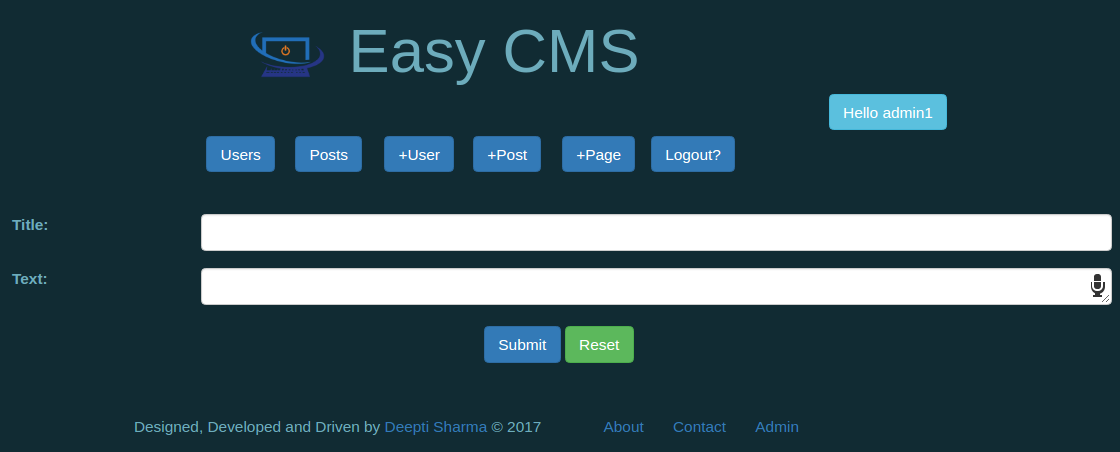
\includegraphics[scale=0.45]{input/images/add.png}                
	\caption{EasyCMS}
	\hspace{-1.5em}
\end{figure}
You may refer to my blogs also for detailed information.\\
Here is the url: \\
https://deepti96.wordpress.com/ \\\\
The interface of EasyCMS looks like this but can be changed using CSS file.
\begin{figure}[!ht]
	\centering
	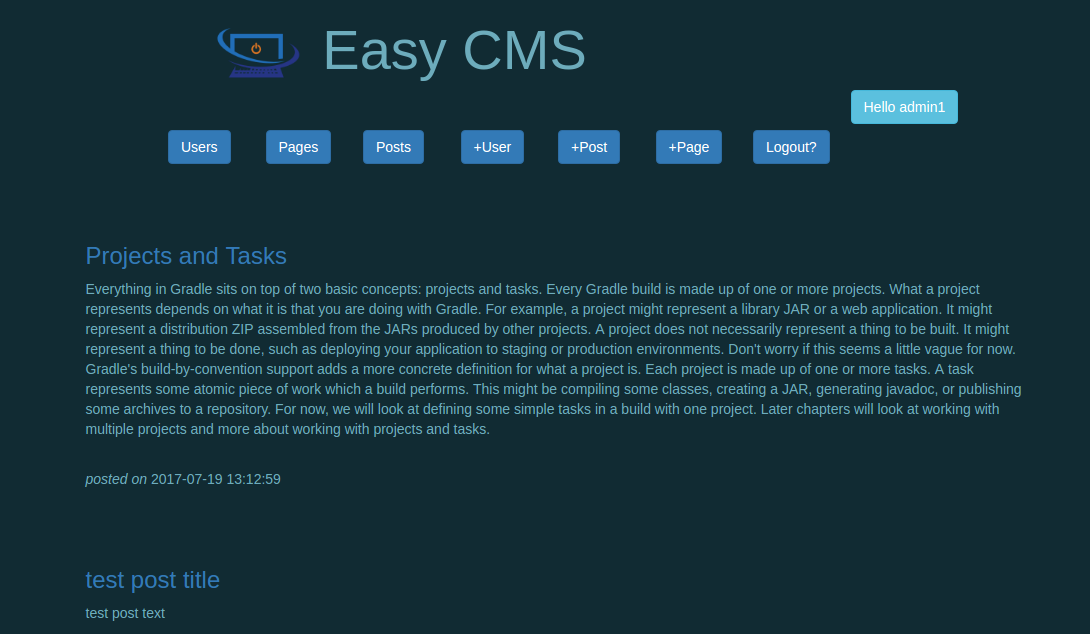
\includegraphics[scale=0.45]{input/images/web.png}                
	\caption{Posted Content}
	\hspace{-1.5em}
\end{figure}\\\\
Contact page of the system: \\
\begin{figure}[!ht]
	\centering
	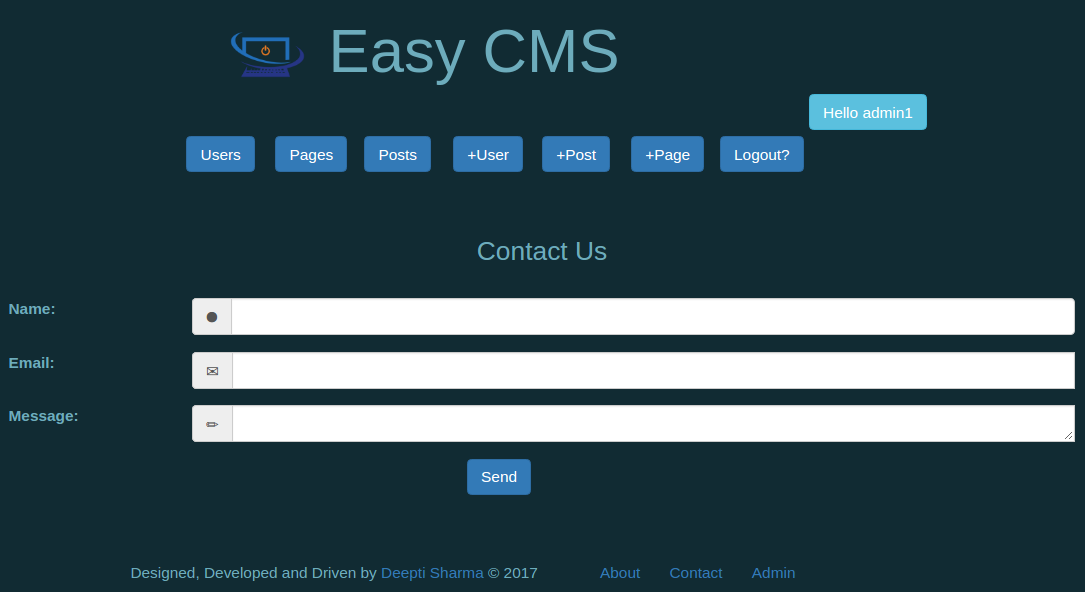
\includegraphics[scale=0.45]{input/images/contact.png}                
	\caption{Contact}
	\hspace{-1.5em}
\end{figure}
\newpage
\subsection{Testing}
Testing a program consists of providing the program with a set of test inputs (or test cases) and
observing if the program behaves as expected. If the program fails to behave as expected, then the
conditions under which failure occurs are noted for later debugging and correction. \\
This software had been taken through rigorous test to fully found potential causes of error and system failure
and full focus have been given to cover all possible exceptions that can 
occur and cause failure of the software.\\
As this software is based on intensive background process it have been taken care that 
if correct input and email address are given then processing of user job can even continue or a least automatically 
restart even after server shuts down or even crash.

\begin{table}[h]
\centering
\begin{tabular}{ ||c|c|| }
\hline
 \multicolumn{2}{||c||}{Overview of CMS} \\
 \hline
 Term & Meaning \\ [0.5ex] 
 \hline \hline
	+Users & Add Users to the Circle \\ \hline
	+Posts & Addition of content by users \\ \hline
	Users & List of Active Users\\ \hline
	Posts & Display published posts. \\ \hline
	+Page & Generate PDF \\ \hline
	Logout &  Logging out        \\ \hline
	
\end{tabular}
\caption{Easy CMS}
\label{table2}
\end{table}

\begin{table}[h]
\centering
\resizebox{\textwidth}{!}{\begin{tabular}{ |c|c|c|c| }
\hline
 \multicolumn{4}{|c|}{Test cases for main page(index.html) } \\[0.5ex]
 \hline
 Input & Desired Output & Actual Output & Status \\ [0.5ex] 
 \hline \hline
 Wrong Credentials & OOPS! Incorrect credentials& OOPS! Incorrect credentials & Pass\\ \hline
 Incorrect User name & Please match the format requested & Please match the format requested & Pass\\ \hline
 No connection & Mailer Error & SMTP connect() failed. & Pass\\ \hline
 Email & Details not sent & Incomplete Email & Pass\\ \hline
 Help needed  & Hello Username & Leads to blog  & Pass\\ \hline
 
\end{tabular}}
\caption{Computational Analysis}
\label{table3}
\end{table}
\begin{table}[h]
\centering
\resizebox{\textwidth}{!}{
\begin{tabular}{ |c|c|c|c| }
\hline
 \multicolumn{4}{|c|}{Test cases for possible source of problems } \\[0.5ex]
 \hline
  Input & Desired Output & Actual Output & Status \\ [0.5ex] 
 \hline \hline 
 URL refreshed & Stick to that page  & Stick at that page only & Pass\\ \hline
 server stops or rebooted & Login Credentials needed & Login Credentials needed & Pass\\ \hline
\end{tabular}}



\caption{Test case (general)}
\label{table}
\end{table}
 
 
 

